\documentclass{article}[14pt]
\usepackage{amsmath}
\usepackage{amsfonts}
\usepackage{graphicx}
\usepackage{enumerate}
\usepackage{dtklogos}
\usepackage{verbatim}
\usepackage{amsmath}
\usepackage{listings}
\usepackage{url}
\usepackage{natbib}
\usepackage{calrsfs}
\usepackage{collectbox}
\usepackage{blindtext}
\newcommand{\R}{{\mathbb R}}
\renewcommand{\vec}[1]{{\mathbf #1}}
\newcommand{\points}[1]{\phantom{.}\hfill \textbf{(#1 points)}}
\newcommand{\matlab}{{\textsc{Matlab}} }



\begin{document}
\begin{center}


\title{Project 1}
\hfill Iliass Tiendrebeogo\\
\hfill ID: 30742742

\bigskip
\hfill \today\\
\end{center}
\bigskip

\begin{center}
  \begin{Large}
      
    Project $N^o 1$ \\
    Math 567: Winter 2016 \\
       
  \end{Large}
\end{center}

\bigskip

\begin{section}
%\item % GOP Nat Primary
{\bf \large 2016 National Republican Primary}

\begin{enumerate}[]

\item % The chart

This is the graphic of 2016 GOP Primary from Feb. 2015. Trends are as follow: Donald Trump's in red curve, Ben Carson's orange curve, Ted Cruz's in green curve, Marco Rubio's show in purple, and the others.

\begin{figure}[h]
\begin{center}
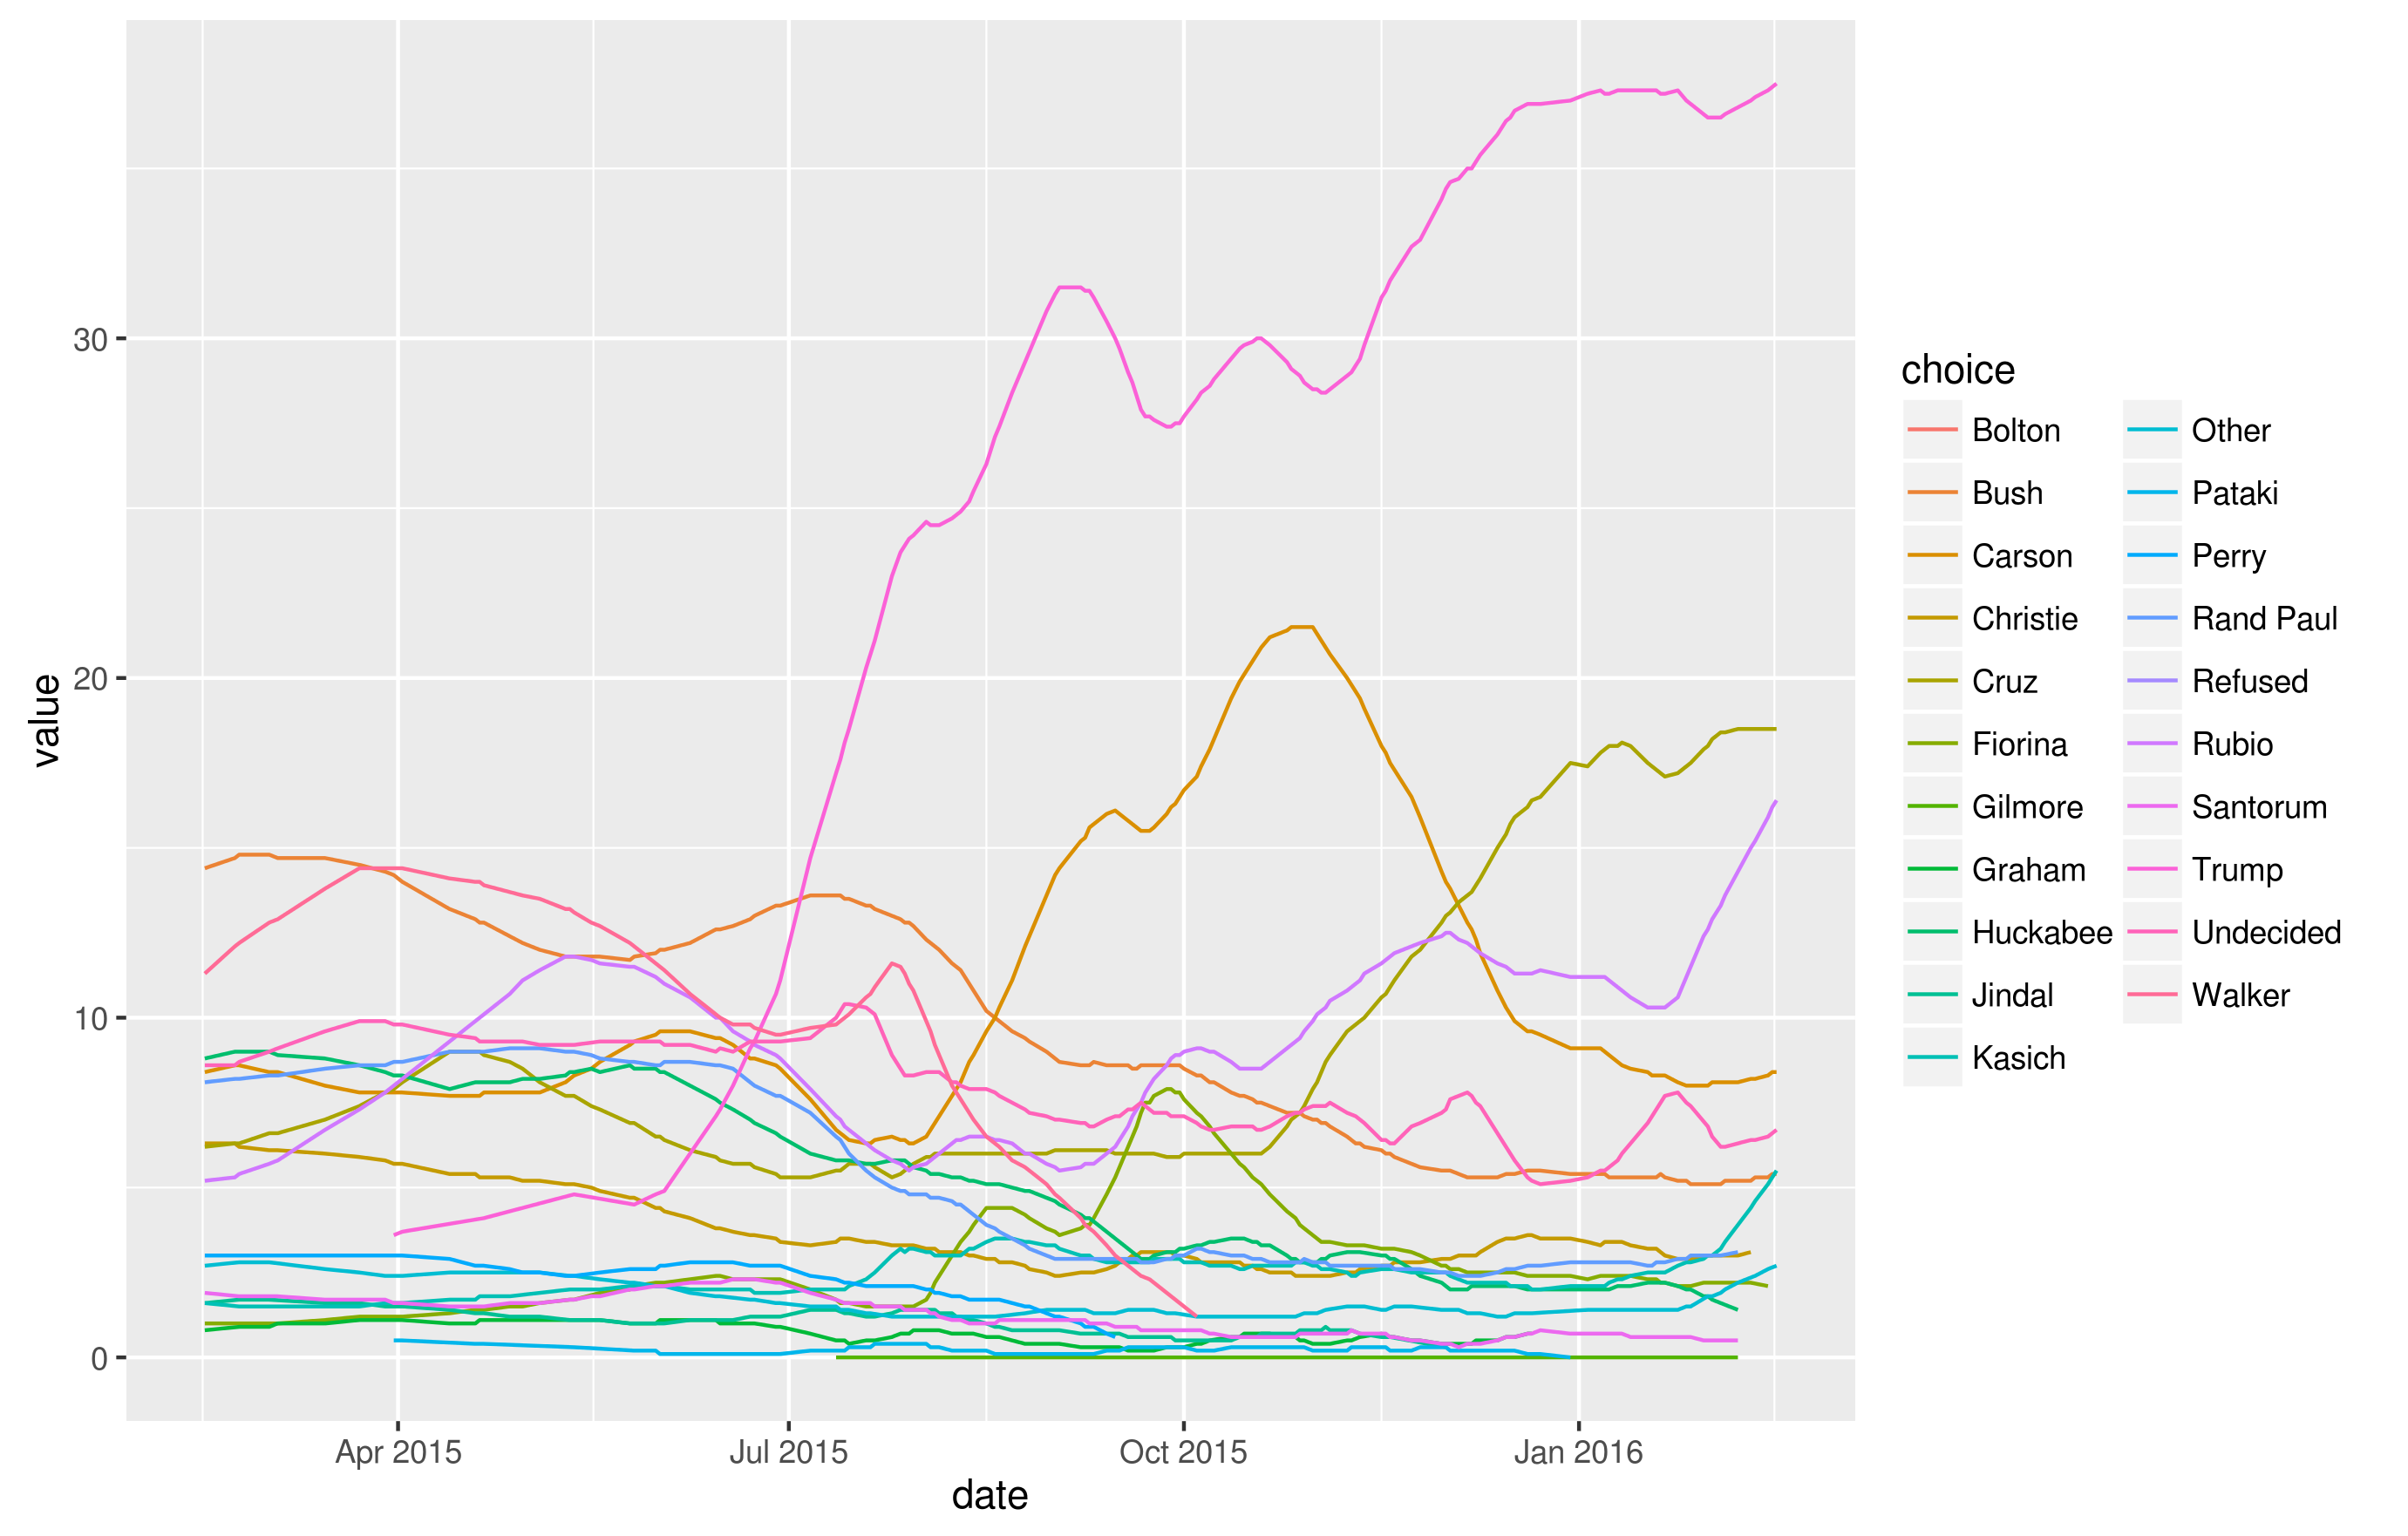
\includegraphics[width=\linewidth]{gop}
\end{center}
\caption{2016 GOP Primary}
\label{fig:figure1}
\end{figure}

A quick view of the chart we can see that there are around six candidates which are still running and only three of them are  relevant. A more in depth analysis show that Donald Trump is leading the race although he got into the race late(April 2015).  He remain unknown during the first two months, before gaining  popularity at a remarkable fast pace and keep growing until now with   $37\%$ today. Whereas, Ben Carson  had lead the second place with a growing popularity from August  to November where his popularity attain a pick at $ 20 \%$ and then drop bellow 10\% for some reasons(which might be related to his declaration about muslims and presidency). And Ted Cruz, who has his popularity below $10\%$ flat since Feb. 2015 have started growing in popularity since November 2015, which might be cause by Ben Carson's falling and Republican need a second runner to trust. The others runners have had a pretty flat popularity which evolve around an average of $10\%$.

One important thing to notice is that lot of Republican Candidates haven't drop out yet.

\item {\bf \large The R Script}


For the entire project we used Huffington post R client by installing the package \cite{Huffpost}

$$ \verb|>install.packages("pollstR")| \\
$$
$$\verb|>library(pollstR)|$$
and the plotting package
$$\verb|> library(ggplot2)|$$
here is the R script:
\begin{lstlisting}[language = R]
we start by loading the  chart data from pollstR
gop_chart <- pollstr_chart('2016-national-gop-primary')

we filter the data frame dy date
gop_frame <- gop_chart[["estimates_by_date"]]

## filtering only from Feb. 2015
gop_frame <- gop_frame[gop_frame$date > as.Date("2015-02-01"),]

## plotting and saving 
gop_plot <- (ggplot(gop_frame, aes(x = date, y = value, color = choice)) + geom_line())
ggsave(file = paste(imageDirectory,"gop.png",sep="/"))
gop_plot
\end{lstlisting}
\end{enumerate}

\end{section}

\bigskip
\begin{section}
%\item % Dem National Primary
{ \bf \large 2016 National Democratic  Primary} 
\bigskip
\begin{enumerate}[]
\item % the chart
The chart on Figure 2 is 2016 National Democratic Primary from Feb. 2015. Trends are as follow: Hillary Clinton's  in yellow curve, Bernie Sander's  in blue curve, and the others.
\begin{figure}[h]
\begin{center}
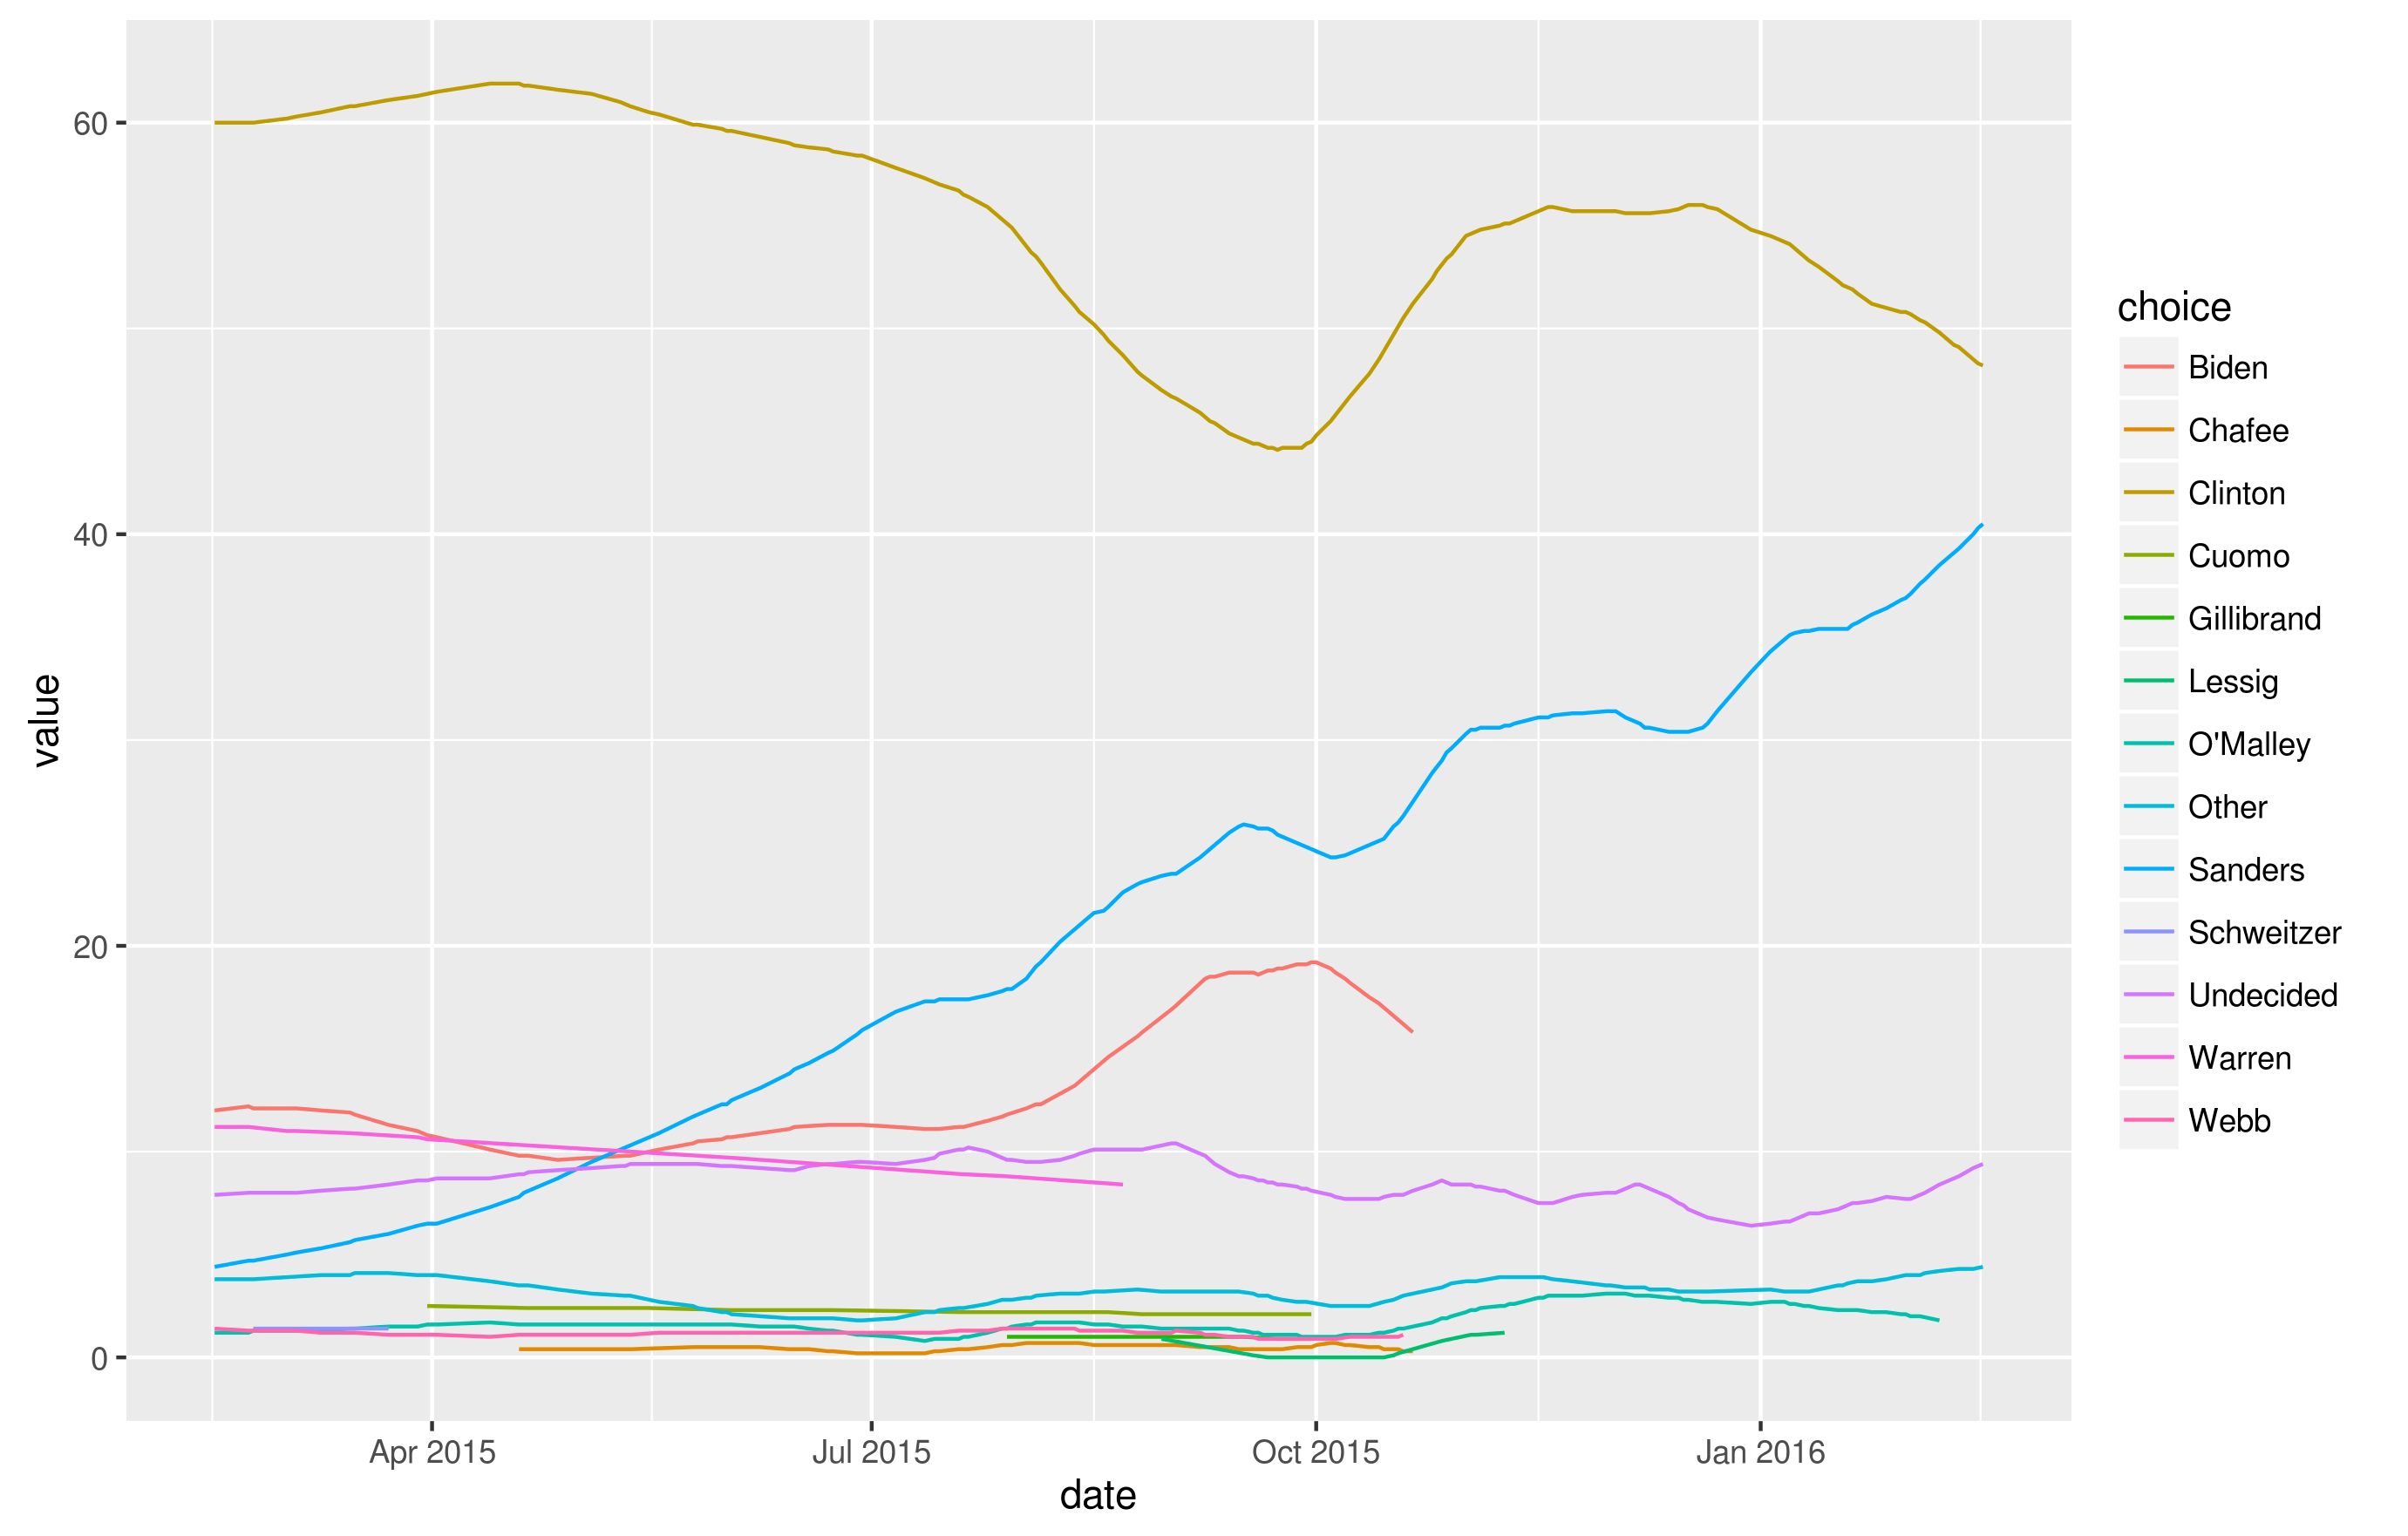
\includegraphics[width=\linewidth]{dem}
\end{center}
\caption{2016 Democratic Primary}
\label{fig:figure 2}
\end{figure}

\medspace
From the chart on Figure 2, we can see that Hillary started astonishingly hight and slowlly decreasing, whereas, Sanders started at the very bottom and going up.

In fact, Hillari's popularity in beginning of 2015 started at around 60\%, it stayed fairly flat until August when her popularity begin decreasing up to a minimal of 44\% in October and then regain some popularity and re-plunge again at 48\% until now. 

In the other hand, Bernie's was literally unknown at the beginning of 2015 with about 4\% popularity, then from March 2015  it start progressing at a fairly fast pace. His progression has been steady since then with no major events up to 40\%.

If we draw a regression line we can clearly see that Hillary's trend has a negative progression even though it is at slower pace. However, a line drawn on Bernie's popularity chart would show a fast positive progression. We are left with the conclusion that if everything stays the same, Bernie Sanders would eventually win the Democratic Party race. But who knows? 

\item {\bf The R Script} % The Scrip


here is the R script:
\begin{lstlisting}[language = R]
we start by loading the  chart data from pollstR
dem_chart <- pollstr_chart('2016-national-democrtic-primary')

we filter the data frame dy date
dem_frame <- dem_chart[["estimates_by_date"]]
# filtering by date from Feb. 2015
dem_frame <- dem_frame[dem_frame$date > as.Date("2015-02-01"),]

# plotting
dem_plot <- (ggplot(dem_frame, aes(x = date, y = value, color = choice))+ geom_line())
ggsave(file = paste(imageDirectory,"dem.png",sep="/"))
dem_plot
\end{lstlisting}
\end{enumerate}

\end{section}

\begin{section}
%\item % SC GOP
{\bf \large 2016 South Carolina Republican Presidential Primary}
\bigskip
\bigskip
\begin{enumerate}[]
\item % the chart
An analisys of the chart we can see that there are around six candidates which are still running and only three of them are  relevant. A more in depth analysis show that Donald Trump is leading the race although he got into the race late(April 2015).  He remain unknown during the first two months, before gaining  popularity at a remarkable fast pace and keep growing until now with   $37\%$ today. Whereas, Ben Carson  had lead the second place with a growing popularity from August  to November where his popularity attain a pick at $ 20 \%$ and then drop bellow 10\% for some reasons(which might be related to his declaration about muslims and presidency). And Ted Cruz, who has his popularity below $10\%$ flat since Feb. 2015 have started growing in popularity since November 2015, which might be cause by Ben Carson's falling and Republican need a second runner to trust. The others runners have had a pretty flat popularity which evolve around an average of $10\%$.
\begin{figure}[h]
\begin{center}
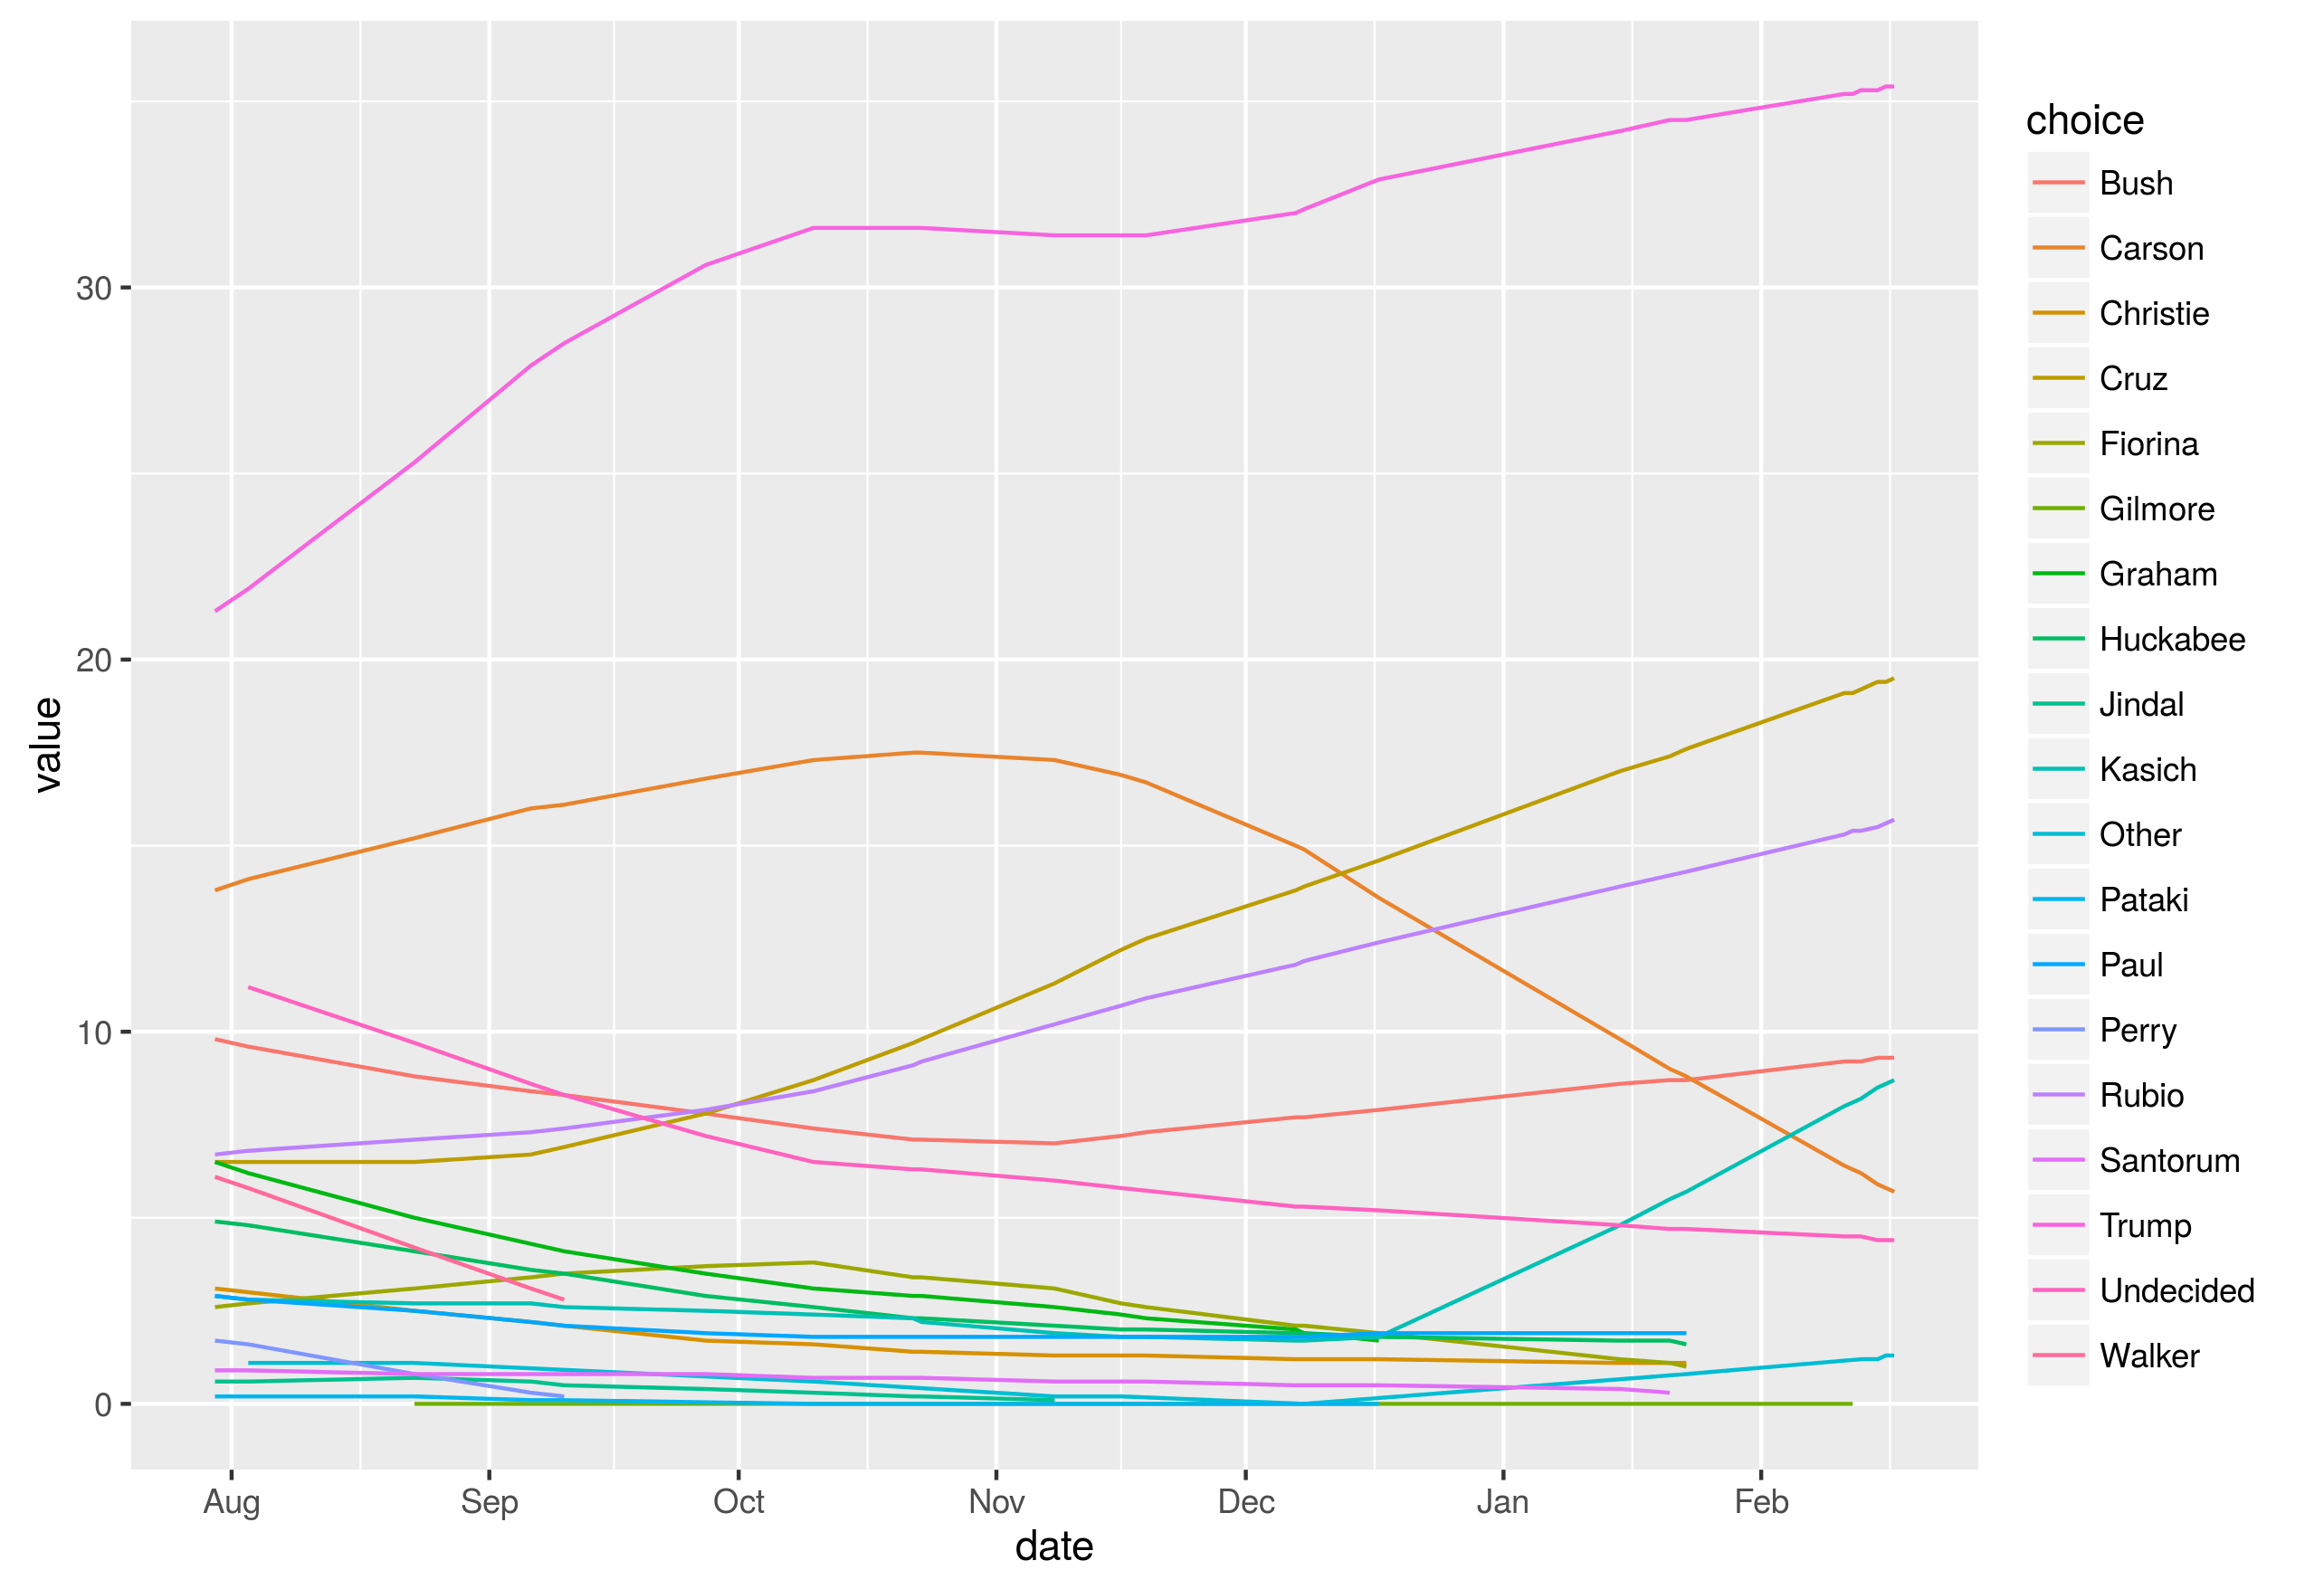
\includegraphics[width=\linewidth]{sc_gop}
\end{center}
\caption{2016 South Crolina GOP Primary}
\label{fig:figure 3}
\end{figure}

\item {\bf The R Script} % The Scrip


here is the R script:
\begin{lstlisting}[language = R]
we start by loading the  chart data from pollstR

sc_polls <- pollstr_polls(chart = slug, after = "2015-07-1", max_pages = 1000000)

sc_questions <-sc_polls[sc_polls$questions$subpopulation == "Likely Voters"] 

plotdata <- merge(sc_polls$polls, sc_questions, by = "id")
## -------- plotting------
sc_plot <- (ggplot(sc_estimates, aes(x = date, y = value, color = choice))+ geom_line())
ggsave(file = paste(imageDirectory,"sc_gop.png",sep="/"))

\end{lstlisting}

\end{enumerate}
\end{section}

\begin{section}
%\item % Obama's Job approval
{\bf \large President Obama's Job Approval}
\begin{enumerate}[]
\item {}


The Chart bellow of Obama's job approval since the start of his Presidency shows in red the approval rate, in green the disapproval rate from late 2008 to February 2016.

\begin{figure}[h]
\begin{center}
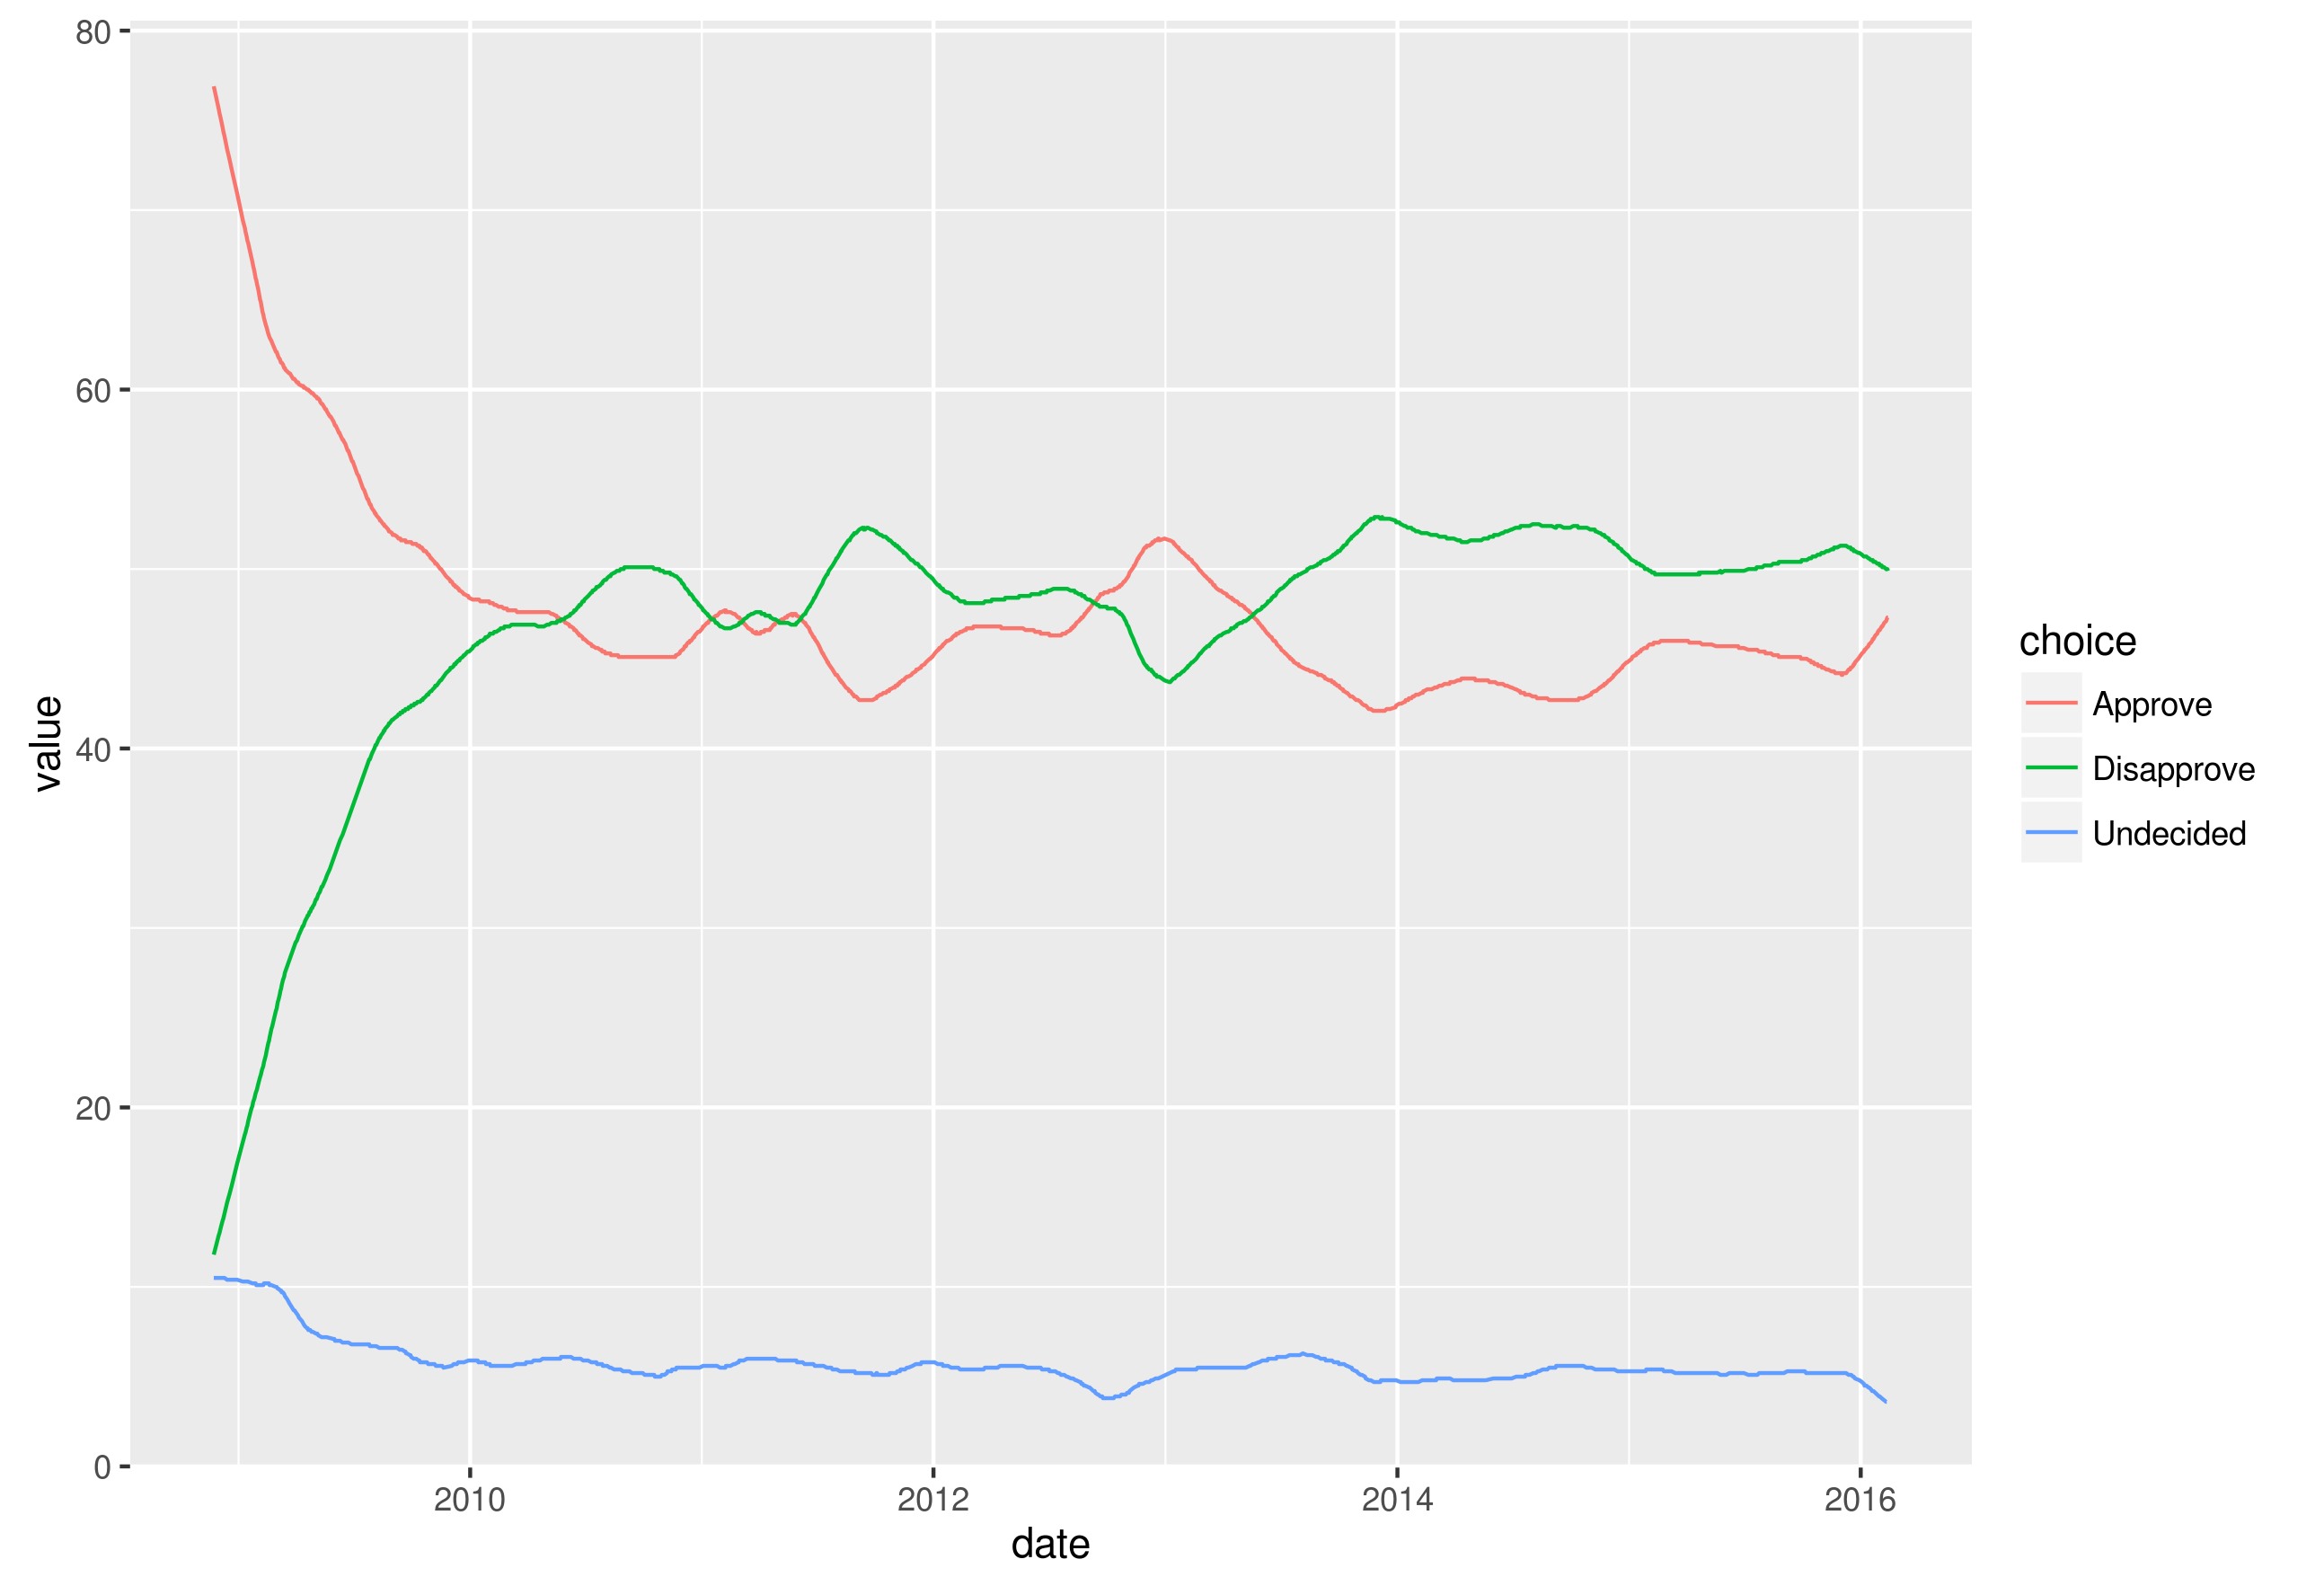
\includegraphics[width=\linewidth]{O_job_app}
\end{center}
\caption{Obama's JOb Approval}
\label{fig:figure4}
\end{figure}

From late 2008 the approval rate start high at about 80 percent, while the disapproval rate start as low as about 15 percent. The approval rate begin to decrease very fast whereas, oppositely the disapproval increased also at a fast rate until early 2010. From 2010 to now those have flatten at about 50 percent with some minor up and down.
\medspace

\item {\bf The Script}

The R Script used to produce this graph is shown bellow

\begin{lstlisting}[language = R]

First we specify the slug, which the topic chart we are interested in to
slug <- "obama-job-approval"

## we generate the chart from pollstR
chart <- pollstr_chart(slug)
estimates <- chart[["estimates_by_date"]]

## we filtered out Undecided
estimates <- estimates[ estimates$choice == "Approve" | estimates$choice == "Disapprove",]

## Ploting 
ggplot(estimates, aes(x = date, y = value, color = choice)) + geom_line()
## we  save into a png file named O_job_approval
ggsave(file = paste(imageDirectory,"O_job_approval.png",sep="/"))
\end{lstlisting}

\end{enumerate}
 
\bigskip
\end{section}

\begin{section}
%\item % Congress Job approval
{\bf \large Congress Job Approval}
\begin{enumerate}[]
\item {} %  the chart

This chart bellow shows the American Congress job approval rating since the beginning of President Obama's presidency. In red is the approval rate and in green the disapproval rate.

\begin{figure}[h]
\begin{center}
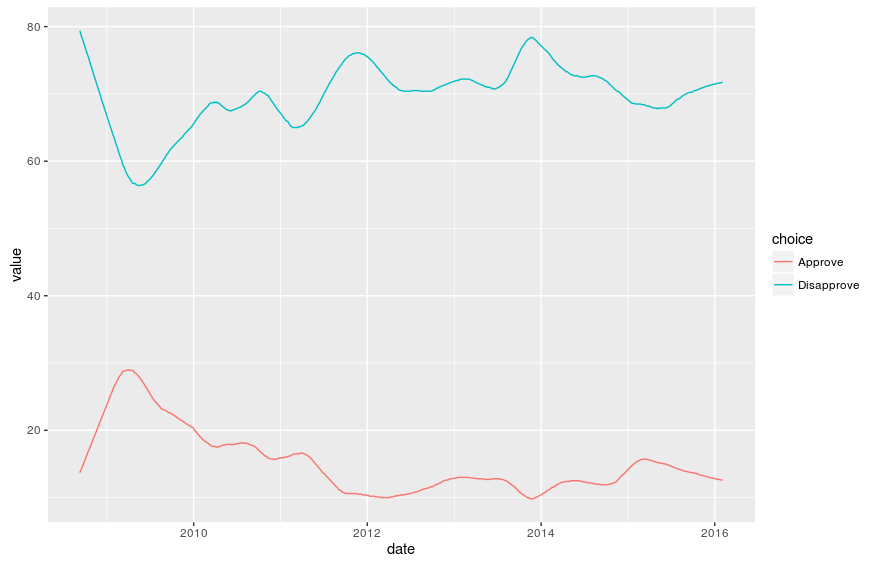
\includegraphics[width=\linewidth]{Congressjobapp}
\end{center}
\caption{Congress Job Approval}
\label{fig:figure 5}
\end{figure}

The analysis of this chart show that from late 2008 the disapproval rate was hight to around 80 percent while the approval rate was very low at about 15 percent. And the approval rate began increasing at a fast pace before attaining his pick at around 30 percent, whereas in the opposite  the disapproval rate started  rapidly decreasing  until attaining a minimal  value of about 55 percent in mid 2009. Then from  2009 to mid 2011 the approval and disapproval rate evolve at a lower pace in opposite direction with an increase of disapproval to about 78 percent and a decrease of approval to around 12 percent. From there those rate have flatten until  now at about the 72 percent an 11 percent.

\item {\large {\bf The Script}}
\begin{lstlisting}[language = R]

First we specify the slug, which the topic chart we are interested in to
slug <- "congress-job-approval"

## we generate the chart from pollstR
chart_congress <- pollstr_chart(slug)

estimates_congress <- chart_congress[["estimates_by_date"]]

## we filtered out Undecided
estimates <- estimates[ estimates$choice == "Approve" | estimates$choice == "Disapprove",]

## filtering by Undecided
estimates_congress <- estimates_congress[ estimates_congress$choice == "Approve" | estimates_congress$choice == "Disapprove",]

# Generate the plot using ggplot2 and save in png file named "Congress_job_app"
ggplot(estimates_congress, aes(x = date, y = value, color = choice)) + geom_line()
ggsave(file = paste(imageDirectory,"Congress_job_app.png",sep="/"))

\end{lstlisting}
\end{enumerate}

\end{section}

\bibliography{Iliass_project_1}
\bibliographystyle{plainnat}
\end{document}